\documentclass[aspectratio=169,fleqn,xcolor={dvipsnames}]{beamer}
\usetheme[pageofpages=of]{hubln}
% dette dokumentet er hoveddokumentet og må kompileres
% resten skjer i Preamble.tex

\usepackage[utf8]{inputenc}
\usepackage[T1]{fontenc}
\usepackage{tabularx}
\usepackage{hhline}
\usepackage{array}
\usepackage{tikz}
\usepackage{amsmath}
\usepackage{amssymb}
\usepackage{tikz-cd}
\usepackage{mathtools}
\usepackage{cancel}
\usepackage{multirow}
\usepackage{minted,xcolor}
\usepackage{caption}
\usepackage{subcaption}
\usemintedstyle{monokai} %vs
%\definecolor{bg}{HTML}{282828}
\definecolor{bg}{RGB}{40, 40, 40}
\setminted{bgcolor=black,frame=lines,
               framesep=2mm}
\usefonttheme{professionalfonts}
\setbeamercovered{invisible}
\hfuzz=8.64pt % Antioverfullbox-inator

\setbeamercolor{block body alerted}{bg=alerted text.fg!10}
\setbeamercolor{block title alerted}{bg=alerted text.fg!20}
\setbeamercolor{block body}{bg=structure!10}
\setbeamercolor{block title}{bg=structure!20}
\setbeamercolor{block body example}{bg=green!10}
\setbeamercolor{block title example}{bg=green!20}
\setbeamertemplate{blocks}[rounded][shadow]


\tikzset{onslide/.code args={<#1>#2}{% from https://tex.stackexchange.com/a/6155/263192
  \only<#1>{\pgfkeysalso{#2}}
}}

\newcommand{\newLine}{%
  \hfill\break
}

\newcommand{\comment}[1]{}
\tikzset{vertex/.style={draw, circle, inner sep=1mm}}
\newcommand{\incomplete}[3][1.5cm]{\begin{tikzpicture}
\foreach \n in {1,...,#2}{\node[vertex]at({90-360/#2*(\n-1)}:#1)(\n){\n};}
\foreach \v/\w in {#3}{\draw(\v)--(\w);}
\end{tikzpicture}}
\tikzset{properties/.style={orange, ultra thick}}
\tikzset{propertiesRed/.style={red, ultra thick}}
\tikzset{propertiesBlue/.style={blue, ultra thick}}
\tikzset{propertiesGrey/.style={gray, ultra thick}}

\usepackage{mathtools}
\DeclarePairedDelimiter\ceil{\lceil}{\rceil}
\DeclarePairedDelimiter\floor{\lfloor}{\rfloor}

% Hier die Daten zur Präsentation eintragen
\author[ls]{Steinar Simonnes og Lukas Schramm}
\title[sgp]{Kræsjkurs MNF130}
\institute{Institutt for informatikk \\ Universitetet i Bergen}
\date[12.05.22]{12 Mai 2022}

\begin{document}
  % Innholdet til selveste presentasjon

% Titel page
\begin{frame}[t,plain]
    \titlepage
\end{frame}

% table of contents (skjer automatisk)
\section{Innføring}
\subsection*{Agenda}
\begin{frame}
    %\tableofcontents
    \begin{columns}[t]
        \begin{column}{.5\textwidth}
            \tableofcontents[sections={1-6}]
        \end{column}
        \begin{column}{.5\textwidth}
            \tableofcontents[sections={7-}]
        \end{column}
    \end{columns}
\end{frame}

\subsection*{Download PDFen}
\begin{frame}{Last meg ned}
    \begin{figure}
        \centering
        \includegraphics[height = 4.9cm]{images/downloadqr.png}
        \caption{https://tinyurl.com/mnf130v22}
        \label{fig:qrcode}
    \end{figure}
\end{frame}

%\input{EksemplerLaTeX}

%===============================================
%Innholdet til selveste presentasjonen
%(1) Logikk - Steinar
%(2) bevis - Steinar
%(9) induksjon - Steinar
%(3) mengdelære/(4) setteory - Steinar
%(5) funksjoner - Steinar
%(12) relasjoner - Steinar
%(6) sekvenser og rekker - Steinar
%
\section{Logikk}
\begin{frame}{Proposisjoner}
\begin{itemize}
    \item En proposisjon er et uttrykk med en sannhetsverdi, som alltid er enten Sann (T) elller Usann (F).
    \item Ofte setter vi dem i variabler, for å gjøre det lettere å lese.
\end{itemize}
\pause
\begin{block}{Proposisjoner}
    p := 2 < 3 \\
    q := ''Månen er laget av ost''\\
    r := ''MNF130 er et nyttig fag for informatikere''
\end{block}
\pause
\begin{block}{Ikke proposisjoner}
    ''Hva skal vi ha til middag i dag?''\\
    x + y < z
\end{block}
\end{frame}

\begin{frame}{$\lnot$, og sannhetstabeller}
\begin{itemize}
    \item Gitt en proposisjon $p$, kan vi representere den motsatte proposisjonen som $\lnot p$.
    \item Vi kan tegne opp alle mulige verdier et slikt uttrykk kan ha i en tabell.
\end{itemize}
\pause

\begin{block}{Eksempler}
    La $p := 2 < 3$. \\
    $p$ = ''Det er sant at 2 er mindre enn 3'' \\
    $\lnot p$ = ''Det er ikke sant at 2 er mindre enn 3''
\end{block}
\pause
\begin{tabular}{c|c}
$p$ & $\lnot p$ \\ \hline
T & F \\
F & T \\ \hline
\end{tabular}
\end{frame}

\begin{frame}{$\lor$ og $\land$}
    \begin{itemize}
        \item Vi kan slå sammen flere proposisjoner til et større uttrykk på mange forskjellige måter.
    \end{itemize}
    \begin{block}{Eksempel}
        La $p$ := Jorden er flat, og $q$ := Månen er flat\\
        $p \lor q$ = Jorden er flat \textbf{eller} månen er flat\\
        $p \land q$ = Jorden er flat \textbf{og} månen er flat\\
    \end{block}
    \pause
    \begin{tabular}{c|c|c|c}
        $p$ & $q$ & $p \lor q$ & $p \land q$ \\ \hline
        T & T & T & T \\
        T & F & T & F \\
        F & T & T & F \\
        F & F & F & F \\
    \end{tabular}
\end{frame}

\begin{frame}{$\rightarrow$ og $\leftrightarrow$}
    \begin{itemize}
        \item En proposisjon kan implisere en annen proposisjon.
    \end{itemize}
    \begin{block}{Eksempel}
        La $p$ := ''Det regner ute'', og $q$ := ''Bakken er våt''\\
        $p \rightarrow q$ = ''Hvis det regner ute, blir bakken våt''\\
        $p \leftrightarrow q$ = ''Det regner ute hvis og bare hvis bakken er våt''
    \end{block}
    \pause
    \begin{tabular}{c|c|c|c}
        $p$ & $q$ & $p \rightarrow q$ & $p \leftrightarrow q$ \\ \hline
        T & T & T & T \\
        T & F & F & F \\
        F & T & T & F \\
        F & F & T & T \\
    \end{tabular}
\end{frame}

\begin{frame}{Ekvivalenser og tautologier}
    \begin{itemize}
        \item Når to logiske uttrykk alltid har samme verdi, sier vi at de er \emph{logisk ekvivalente}.
        \item Om et uttrykk alltid er sant, uavhengig av innholdet, kaller vi det en tautologi.
    \end{itemize}
    \begin{tabular}{c|c|c|c}
         $p$ & $\lnot p$ & $\lnot \lnot p$ & $p \lor \lnot p$\\ \hline
         T & F & T & T\\
         F & T & F & T
    \end{tabular}
    \pause
    \begin{itemize}
        \item Konklusjon 1: $p \equiv \lnot \lnot p$
        \pause
        \item Konklusjon 2: $p \lor \lnot p \equiv T$, og er en tautologi
        \pause
        \item For å se om to uttrykk er ekvivalente, tegn sannhetstabellen og se om kollonene deres er det samme.
        \item For å se om et uttrykk er en tautologi, tegn sannhetstabellen og se om kolonnen alltid er T.
    \end{itemize}
\end{frame}

\begin{frame}{Noen viktige logiske ekvivalenser}
    \begin{columns}
    \begin{column}{0.32\textwidth}
        \begin{tabular}{l|c}
        Ekvivalens & Navn \\ \hline
        $p \land T \equiv p$ & Identity\\
        $p \lor F \equiv p$ \\ \hline
        
        $p \lor T \equiv T$ & Domination\\
        $p \land F \equiv F$\\ \hline
        
        $p \lor p \equiv p$ & Idempotent\\
        $p \land p \equiv p$ \\ \hline
        
        $p \equiv \lnot \lnot p$ & Negation\\ \hline
        
        $p \lor q \equiv q \lor p$ & Commutative\\
        $p \land q \equiv q \land p$ \\
        

    \end{tabular}
    \end{column}
    \begin{column}{0.52\textwidth}
        \begin{tabular}{l|c}
        Ekvivalens & Navn \\ \hline
        
        $(p \lor q) \lor r \equiv p \lor (q \lor r)$ & Associative\\
        $(p \land q) \land r \equiv p \land (q \land r)$ \\ \hline
        
        $p \lor (q \land r) \equiv (p \lor q) \land (p \lor r)$ & Distributive\\
        $p \land (q \lor r) \equiv (p \land q) \lor (p \land r)$ \\ \hline
        
        $\lnot (p \land q) \equiv \lnot p \lor \lnot q$ & De Morgan \\
        $\lnot (p \lor q) \equiv \lnot p \land \lnot q$ \\ \hline
        
        $p \lor (p \land q) \equiv p$ & Absorption \\
        $p \land (p \lor q) \equiv q$ \\ \hline
        
        $p \lor \lnot p \equiv T$ & Negation \\
        $p \land \lnot p \equiv F$ \\
        \end{tabular}
    \end{column}
\end{columns}
\end{frame}

\begin{frame}{Flere viktige logiske ekvivalenser}
    \begin{columns}
    \begin{column}{0.48\textwidth}
        \begin{tabular}{c}
            Ekvivalenser med $\rightarrow$ \\ \hline
            $p \rightarrow q \equiv \lnot p \lor q$ \\
            $p \rightarrow q \equiv \lnot p \rightarrow \lnot q$ \\
            $p \lor q \equiv \lnot p \rightarrow q$ \\
            $p \land q \equiv \lnot (p \rightarrow \lnot q)$ \\
            $\lnot (p \rightarrow q) \equiv p \land \lnot q$ \\
            $(p \rightarrow q) \land (p \rightarrow r) \equiv p \rightarrow (q \land r)$ \\
            $(p \rightarrow q) \land (q \rightarrow r) \equiv (p \lor q) \rightarrow r$ \\
            $(p \rightarrow q) \lor (p \rightarrow r) \equiv p \rightarrow (q \lor v)$ \\
            $(p \rightarrow r) \lor (q \rightarrow r) \equiv (p \land q) \rightarrow r$
        \end{tabular}
    \end{column}
    \begin{column}{0.48\textwidth}
        \begin{tabular}{c}
            Ekvivalenser med $\leftrightarrow$ \\ \hline
            $p \leftrightarrow q \equiv p \rightarrow q \land q \rightarrow p$ \\
            $p \leftrightarrow q \equiv \lnot p \leftrightarrow \lnot q$ \\
            $p \leftrightarrow q \equiv (p \land q) \lor (\lnot p \land \lnot q)$\\
            $\lnot (p \leftrightarrow q) \equiv p \rightarrow \lnot q$
        \end{tabular}
    \end{column}
    \end{columns}
\end{frame}

\begin{frame}{Typisk logikkoppgave}
    \begin{columns}
    \begin{column}{0.48\textwidth}
        Vis at $(p \land \lnot q) \rightarrow \lnot r$ og $(p \land r) \rightarrow q$ er logisk ekvivalente, ved å bruke enkle logiske ekvivalenser.\\[1cm]
        
        1. $a \rightarrow b \equiv \lnot a \lor b$ \\
        2. $\lnot (a \land b) \equiv \lnot a \lor \lnot b$\\
        3. $\lnot (\lnot a) \equiv a$
    \end{column}
    \begin{column}{0.48\textwidth}
        \begin{math}
            \pause
            (p \land q) \rightarrow \lnot r \\
            \pause
            \equiv \lnot (p \land \lnot q) \lor \lnot r \\
            \pause
            \equiv (\lnot p \lor \lnot \lnot q) \lor \lnot r \\
            \pause
            \equiv (\lnot p \lor q) \lor \lnot r \\
            \pause
            \equiv \lnot p \lor q \lor \lnot r \\
            \pause
            \equiv \lnot p \lor \lnot r \lor q \\
            \pause
            \equiv \lnot (p \land r) \lor q \\
            \pause
            \equiv (p \land r) \rightarrow q
            \qed
        \end{math}
    \end{column}
    \end{columns}
\end{frame}

\begin{frame}{Predikater}
    \begin{itemize}
        \item Et predikat er bare en funksjon som returnerer T eller F.
        \item Gitt et predikat og riktig antall argumenter, kan vi evaluere det som en vanlig proposisjon.
    \end{itemize}
    \begin{block}{Eksempler på predikater}
        $P(x, y, z) = x + y < z$\\
        $Q(s)$ = $s$ contains $'a'$
    \end{block}
    \pause
    \begin{block}{Eksempler på evaluering}
        $P(1, 2, 3) = 1 + 2 < 3 = F$ \\ 
        $Q(''Steinar'') = ''Steinar''$ contains $'a' = T$
    \end{block}

\end{frame}

\begin{frame}{Kvantorer (/Quantifiers)}
    \begin{itemize}
        \item Ofte vil vi si noe om et predikat $P(x)$, men for flere potensielle $x$ samtidig.
        \item $\forall x P(x)$ = ''For alle $x$ er det sant at $P(x)$''
        \item $\exists x P(x)$ = ''Det eksisterer en $x$ slik at det er sant at $P(x)$''
    \end{itemize}
    
    \pause
    \begin{block}{Eksempler}
        $\forall x (x < x + 1)$ = ''For alle x er det sant at $x < x +1$''\\[5mm]
        $\exists x (x > x^2)$ = ''Det eksisterer en x slik at det er sant at $x > x^2$''
    \end{block}
\end{frame}

\begin{frame}[fragile]{Kvantorer i praksis}
    \begin{minted}[fontsize=\scriptsize]{python}
def forall(p, xs):
    for x in xs:
        if not p(x):
            return False
    return True
    
def exists(p, xs):
    for x in xs:
        if p(x):
            return True
    return False
    \end{minted}
    
    \pause
    \begin{itemize}
        \item exists(p, xs) = $\exists x (x \in xs \land p(x))$
        \item forall(p, xs) = $\forall x (x \in xs \land p(x))$
    \end{itemize}
\end{frame}

\begin{frame}{Nøstede kvantorer (/Nested quantifiers)}
    \begin{itemize}
        \item Ofte vil vi si noe om mange kombinasjoner av variabler samtidig.
        \item Da slår vi sammen flere $\forall$ og $\exists$.
    \end{itemize}
    
    \begin{block}{Eksempler}
        $\forall x \forall y (x^2 + y^2 \geq 0)$ \\
        $\forall x \exists y (x * y = 1)$ = ''For alle x eksisterer det en y slik at er $x * y = 1$'' \\
        $\exists x \forall y (x^2 < y^2)$ = ''Det eksisterer en x slik at for alle y er $x^2 \leq y^2$''\\
        $\lnot \exists n \exists a \exists b \exists c (a,b,c,n \in Z \land n > 2 \land a^n + b^n = c^n)$
    \end{block}
\end{frame}

\begin{frame}{De Morgan dukker opp igjen}
Det viser seg at De Morgan's lover også fungerer på kvantorer.\\
    \begin{columns}
    \begin{column}{0.48\textwidth}
    \begin{itemize}
        \item $\lnot \forall x P(x) \equiv \exists x \lnot P(x)$
        \item $\lnot \exists x P(x) \equiv \forall x \lnot P(x)$
    \end{itemize}        
    \end{column}
    \pause
    \begin{column}{0.48\textwidth}
        \includegraphics[scale=0.3]{Always a bigger fish.jpeg}
        \pause
        \includegraphics[scale=1]{bigger fish.PNG}
    \end{column}
    \end{columns}
    

\end{frame}

\subsection*{Spørretid}
\begin{frame}{Spørsmål?}
    \begin{figure}
        \centering
        \includegraphics[height = 4.9cm]{images/guillaume5.jpg}
        \caption{Guillaume på Vidden}
        \label{fig:guillaume5}
    \end{figure}
\end{frame}

\section{Mengdelære og funksjoner}
\begin{frame}{Sett / Mengder}
    Et sett, eller en mengde, er en kolleksjon av objekter med to regler:\\
    \indent \hspace{3mm}    1. Det inneholder ingen duplikater\\
    \indent \hspace{3mm}    2. Det har ingen konkret rekkefølge
    
    \pause
    \begin{block}{Eksempel}
        Alle de følgende settene er like: \\
        $\{1, 2, 3\}$, $\{3, 2, 1\}$ \\
        $\{1, 1, 1, 1, 2, 2, 3, 3\}$
    \end{block}
    
    \pause
    \begin{block}{Eksempel}
        $1 \in \{1, 2, 3\}$ = T \\
        $5 \in \{1, 2, 3\}$ = F
    \end{block}
\end{frame}


\begin{frame}{Kjente sett}
    Flere sett bruker vi veldig ofte. Her er noen av dem.\\
    
    \begin{tabular}{c|l|c}
        Symbol & Navn & Innhold \\ \hline
        $\mathbb{N}$ & Naturlige tall & $\{0, 1, 2, 3, ....\}$\\
        $\mathbb{Z}$ & Heltall & $\{... -2, -1, 0, 1, 2, 3, ....\}$\\
        $\mathbb{Q}$ & Rasjonale tall & $\{-3/2, 1/10, 4/5, 5/4, ....\}$\\
        $\mathbb{R}$ & Reelle tall & $\{\pi, e, 0.111111111..., 2*\pi, .....\}$\\
        $\emptyset$ & Det tomme settet & $\{\}$
    \end{tabular}
    
\end{frame}

\begin{frame}{Settbyggingsnotasjon}
    Istedet for å manuelt skrive opp alle elementene i et sett, eller å bruke uformell \enquote{...}-notasjon, kan vi bruke setbyggingsnotasjon.
    \begin{block}{Eksempler}
        $\{ n | n \in \mathbb{N}\}$ = $\mathbb{N}$\\
        $\{ n \cdot 2 | n \in \mathbb{N}\}$ = $\{0, 2, 4, 6, 8, ....\}$\\
        $\{ i / 2 | i \in \mathbb{N}, i$ mod $3 = 0\}$ = $\{0, 1.5, 3, 4.5, 6, ...\}$
    \end{block}
\end{frame} 

\begin{frame}{$\cup$, $\cap$, $\bar{}$ og $-$}
    $A \cup B := \{x | x \in A \lor x \in B\}$ \\
    $A \cap B := \{x | x \in A \land x \in B\}$\\
    $A - B = A \backslash B := \{x | x \in A\land  x \notin B\}$\\
    $A^C = \bar{A} := \{x | x \notin A\}$
    
    \pause
    \begin{figure}%
        \centering
        \subfloat[\centering $A \cup B$]{{\includegraphics[width=2.5cm]{union.png} }}%
        \qquad
        \subfloat[\centering $A \cap B$]{{\includegraphics[width=2.5cm]{snitt.png} }}%
        \qquad
        \subfloat[\centering $B - A$]{{\includegraphics[width=2.5cm]{minus.png} }}%
        \qquad
        \subfloat[\centering $\bar{A}$]{{\includegraphics[width=2.5cm]{complement.png} }}%
        % \caption{Vennediagramer}%
        \label{fig:example2}%
    \end{figure}
\end{frame}

\begin{frame}{$\subset, \subseteq, =, \supseteq, \supset$}
    Vi har flere måter å uttrykke at et sett inneholder elementer fra et annet sett.
    \begin{itemize}
        \item $A \subseteq B := \forall x (x \in A \rightarrow x \in B)$
        \item $A \supseteq B := B \subseteq A$
        \item $A \subset B := \forall x (x \in A \rightarrow x \in B) \land \exists y (y \in B \land y \notin A)$
        \item $A \supset B := B \subset A$
        \item $A = B := A \subseteq B \land B \subseteq A$
    \end{itemize}
    \pause
    \begin{block}{Eksempler}
        $\{1\} \subseteq \{1, 2\}$ = T\\
        $\{1\} \subseteq \{5\}$ = F\\
        $\{a, b\} \subset \{a, b\}$ = F\\
        $\{a, b\} \subseteq \{a, b\}$ = T
    \end{block}
    
\end{frame}

\begin{frame}{Tavleoppgaver fra H19}
    \begin{itemize}
        \item Vis eller motbevis at $(A - C) \cap (B - C) = \emptyset.$
        \item Vis eller motbevis at $(A - C) \cap (C - B) = \emptyset.$
    \end{itemize}
    
    For å løse det med vennediagrammer:
    \begin{itemize}
        \item Tegn et vennediagram. Begynn med sirkler for A, B, etc.
        \item Farg inn (helst med forskjellige farger) områdene til deluttrykkene, dvs $(A - C)$ eller $(B - C)$ i dette eksemplet.
        \item Bruk områdene i deluttrykkene til å farge omårdene i de større uttrykkene, dvs hele $(A - C) \cap (B - C)$ her.
        \item Er områdene til hele uttrykkene på hver side av = det samme?
    \end{itemize}
    \pause
    Alternativt: bruk definisjonene til $\cap$, $\cup$, etc til å omformulere uttrykket til det på høyresiden av =.
\end{frame}

\begin{frame}{Nyttige regler for sett}
        \begin{tabular}{l|c}
        Ekvivalens & Navn \\ \hline
        $A \cap U = A$ & Identity\\
        $A \cup \emptyset = A$ \\ \hline
        
        $A \cup U = U$ & Domination\\
        $A \cap \emptyset = \emptyset$\\ \hline
        
        $A \cup A = A$ & Idempotent\\
        $A \cap A = A$ \\ \hline
        
        $A = (A^C)^C$ & Negation\\ \hline
        
        $A \cup B = B \cup A$ & Commutative\\
        $A \cap B = B \cap A$ \\

    \end{tabular}
    \hfill
        \begin{tabular}{l|c}
        Ekvivalens & Navn \\ \hline
        
        $(A \cup B) \cup C = A \cup (B \cup C)$ & Associative\\
        $(A \cap B) \cap C = A \cap (B \cap C)$ \\ \hline
        
        $A \cup (B \cap C) = (A \cup B) \cap (A \cup C)$ & Distributive\\
        $A \cap (B \cup C) = (A \cap B) \cup (A \cap C)$ \\ \hline
        
        $(A \cap B)^C = A^C \cup B^C$ & De Morgan \\
        $(A \cup B)^C = A^C \cap B^C$ \\ \hline
        
        $A \cup (A \cap B) = A$ & Absorption \\
        $A \cap (A \cup B) = A$ \\ \hline
        
        $A \cup A^C = U$ & Negation \\
        $A \cap A^C = \emptyset$ \\
        \end{tabular}
\end{frame}

\begin{frame}{Funksjoner}
    Funksjoner kjenner vi fra INF100 i fjor. Nå skal vi formalisere dem litt mer.\\
    Se på funksjoner som en utregning fra et eller flere sett til et annet sett.\\
    Domenet til en funksjon er inputsettet.\\
    Kodomenet til en funksjon er outputsettet.\\
    %\begin{block}
    \pause
    \begin{columns}
    \begin{column}{0.25\textwidth}
         $f : \mathbb{R} \rightarrow \mathbb{R}$\\
        $f(x) := x+1$ \\
        
        $P : (\mathbb{R}, \mathbb{R}) \rightarrow Bool$\\
        $P(x, y) := x^2 < y$
     \end{column}
    \begin{column}{0.35\textwidth}
         $$
            g : \mathbb{Z} \rightarrow Bool \\
            g(n) :=
            \begin{cases}
            T, n \text{ mod } 2 = 0\\
            F, \text{otherwise}\\
            \end{cases}
        $$
    \end{column}
    \end{columns}
    %\end{block}
\end{frame}

\begin{frame}{Injektivitet, Surjektivitet}
    En funksjon $f : A \rightarrow B$ er:
    \begin{itemize}
        \item Injektiv hvis $\forall a_1 \forall a_2 (f(a_1) = f(a_2) \rightarrow a_1 = a_2)$.     Med andre ord: alle inputs gir et unikt output.\\
        \item Surjektiv hvis $\forall b \exists a (f(a) = b)$. Med andre ord: alle $b$ har minst én representant i $A$.
        \item Bijektiv hvis den er både injektiv og surjektiv. Da har den et invers.
    \end{itemize}
    \pause
    \begin{figure}%
        \centering
        \subfloat[\centering $Injektiv$]{{\includegraphics[width=2.5cm]{inj.png} }}%
        \qquad
        \subfloat[\centering $Surjektiv$]{{\includegraphics[width=2.5cm]{sur.png} }}%
        \qquad
        \subfloat[\centering $Bijektiv$]{{\includegraphics[width=2.5cm]{bi.png} }}%
        \qquad
        \subfloat[\centering $Ingenting$]{{\includegraphics[width=2.5cm]{nothing.png} }}%
        \label{fig:example1}%
    \end{figure}
\end{frame}

\begin{frame}{Injektivitet, Surjektivitet}
    \begin{itemize}
        \item Injektiv:  $\forall a_1 \forall a_2 (f(a_1) = f(a_2) \rightarrow a_1 = a_2)$.\\
        \item Surjektiv: $\forall b \exists a (f(a) = b)$.\\
        \item Bijektiv: begge de over \\
    \end{itemize}
    \pause
    \begin{block}{Avgjør om de følgende funksjonene er injektive, surjektive, eller bijektive:}
        $f : \mathbb{R} \rightarrow \mathbb{R}$, $f(x) := 2x + 1$\\
        $g : \mathbb{Z} \rightarrow $ Bool, $g(x) := x$ mod $2 = 0$\\
        $h : \mathbb{R} \rightarrow \mathbb{R}$, $h(x) := e^x$\\
        $k : \mathbb{R} \rightarrow \mathbb{R^+}$, $k(x) := e^x$\\
    \end{block}
\end{frame}

\begin{frame}{Funksjonskomposisjon}
    \begin{columns}
    \begin{column}{0.5\textwidth}
Gitt to funksjoner:
    \begin{itemize}
        \item $f : A \rightarrow B$
        \item $g : B \rightarrow C$
    \end{itemize}
Kan vi definere en unik tredje funksjon: \\
    $g \circ f : A \rightarrow C$\\
    $g \circ f := g(f(x))$\\
    \pause
Om en funksjon $f : A \rightarrow B$ er bijektiv, finnes det en unik invers funksjon $f^{-1} : B \rightarrow A$ slik at $f(f^{-1}(x)) = x$ og $f^{-1}(f(x)) = x$.
    \end{column}
    \begin{column}{0.33\textwidth}
    \begin{figure}
       \includegraphics[scale = 0.4]{gof.jpeg} 
    \end{figure}
        
    \end{column}
    \end{columns}
\end{frame}

\begin{frame}{Kardinalitet}
    Om $A$ er et sett, er $|A|$ antall elementer i settet, \textit{kardinaliteten}, eller \textit{lengden}.\\
    To sett har samme kardinalitet om de har samme lengde. Da finnes det en bijeksjon mellom settene.
    \begin{block}
        $|\{a, b, c\}| = 3$\\
        $|\{\}| = 0$\\
        $|\mathbb{N}| = \aleph_0$
    \end{block}
\end{frame}

\begin{frame}{Tellbarhet}
    \begin{columns}
    \begin{column}{0.48\textwidth}
        Hva er størst av $|\mathbb{N}|$ og $|\mathbb{Z}|$?\\
        \pause
        f(n) :=
        \begin{cases}
            \frac{n}{2}, n \text{ mod } 2 = 0\\
            -\frac{n+1}{2}, \text{otherwise}\\
        \end{cases}\\
        \pause
        Konklusjon: $|\mathbb{N}|$ = $|\mathbb{Z}|$ = $\aleph_0$.
    \end{column}
    \pause
    \begin{column}{0.48\textwidth}
        Hva er størst av $|\mathbb{N}|$ og $|\mathbb{Q}|$?\\
        \pause
        $f(0) := 1$\\
        $f(n) := \frac{1}{2\lfloor f(n-1) \rfloor - f(n-1)+1}$\\
        $g(0) := 0$\\
        $g(2n) := f(n)$\\
        $g(2n-1) := -f(n)$\\
        \pause
        Konklusjon: $|\mathbb{N}|$ = $|\mathbb{Q}|$ = $\aleph_0$
    \end{column}
    \end{columns}\\
    
    \pause
    \newline Derimot er $|\mathbb{R}| > |\mathbb{N}|$. For en enkel forklaring med et eksempel, se Veritasiums video om Hilberts Hotell: \url{https://www.youtube.com/watch?v=OxGsU8oIWjY}
    
%Gud, alle disse feilmeldingene, Steinar
\end{frame}

\subsection*{Spørretid}
\begin{frame}{Spørsmål?}
    \begin{figure}
        \centering
        \includegraphics[height = 4.9cm]{images/guillaume4.jpg}
        \caption{Guillaume på Vidden}
        \label{fig:guillaume4}
    \end{figure}
\end{frame}

\section{Relasjoner}
\begin{frame}[fragile]{Relasjoner}
    En relasjon fra $A$ til $B$ er et subset av $A \times B$.\\
    \pause
    De er lettere å visualisere ved å tegne dem:\\
    
    R := $\{(a, b), (b, b), (d, c), (d, b), (a, c)\}$\\
\begin{tikzcd}
a \arrow[rr] \arrow[rrdd] &  & b \arrow[loop, distance=2em, in=305, out=235] \\
                          &  &                                               \\
d \arrow[rr] \arrow[rruu] &  & c                                            
\end{tikzcd}

\pause
Veldig ofte er $A$ og $B$ det samme settet, dvs at $R$ er et subset av $A \times A$. Da kaller vi R en relasjon \emph{på} $A$.
\end{frame}

\begin{frame}[fragile]{Praktisk eksempel på en relasjon}
    La objektene være alle typer i Python. \\
    La det være en relasjon fra $a$ til $b$ om det finnes en funksjon fra typen $a$ til typen $b$.\\
    
\begin{tikzcd}
Int \arrow[rr, ''bool()'', bend right] \arrow[dd, ''str()'', bend left] &  & Bool \arrow[lldd, ''str()''] \arrow[ll, ''int()''', bend right] \\
                                                                    &  &                                                             \\
Str \arrow[rr, ''.split()''] \arrow[uu, ''int()'', bend left]           &  & {[Str]}                                                    
\end{tikzcd}
\end{frame}

\begin{frame}{Forskjellige typer relasjoner}
Gitt en relasjon $R \subseteq A \times A$ på $A$ har vi 5 viktige begreper for å beskrive den:
    \begin{itemize}
        \item Refleksiv: $\forall a ((a, a) \in R)$
        \pause
        \item Symmetrisk: $\forall a \forall b ((a, b) \in R \leftrightarrow (b, a) \in R)$
        \pause
        \item Antisymmetrisk: $\forall a \forall b ((a, b) \in R \land (b, a) \in R \rightarrow a = b)$
        \pause
        \item Transitiv: $\forall a \forall b \forall c [(a, b) \in R \land (b, c) \in R \rightarrow (a, c) \in R]$\\
        \pause
        \item Om en relasjoner er refleksiv, symmetrisk og transitiv, kaller vi det en ekvivalensrelasjon.
    \end{itemize}   
\end{frame}

\begin{frame}[fragile]{Refleksive relasjoner}
En relasjon $R$ er refleksive hvis $\forall a ((a, a) \in R)$.\\
    \begin{columns}
        \begin{column}{0.3\textwidth}
        Ikke refleksiv:
            \begin{tikzcd}
a \arrow[dd] \arrow[rr] &  & b                                             \\
                        &  &                                               \\
c \arrow[rruu]          &  & d \arrow[loop, distance=2em, in=305, out=235]
\end{tikzcd}
        \end{column}
        \pause
        \begin{column}{0.3\textwidth}
        
Refleksiv:
\begin{tikzcd}
a \arrow[dd] \arrow[rr] \arrow[loop, distance=2em, in=305, out=235] &  & b \arrow[loop, distance=2em, in=305, out=235] \\
                                                                    &  &                                               \\
c \arrow[rruu] \arrow[loop, distance=2em, in=305, out=235]          &  & d \arrow[loop, distance=2em, in=305, out=235]
\end{tikzcd}
        \end{column}
    \end{columns}
\end{frame}

\begin{frame}[fragile]{Symmetriske relasjoner}
En relasjon $R$ er symmetrisk hvis $\forall a \forall b ((a, b) \in R \leftrightarrow (b, a) \in R)$.\\
    \begin{columns}
        \begin{column}{0.3\textwidth}
            Ikke symmetrisk:\\
            \begin{tikzcd}
a \arrow[dd]   &  & b                                             \\
               &  &                                               \\
c \arrow[rruu] &  & d \arrow[loop, distance=2em, in=305, out=235]
\end{tikzcd}
        \end{column}
        \pause
        \begin{column}{0.3\textwidth}
    
        Symmetrisk:
        \begin{tikzcd}
a \arrow[dd, bend left]                          &  & b \arrow[lldd, bend right]                    \\
                                                 &  &                                               \\
c \arrow[rruu, bend right] \arrow[uu, bend left] &  & d \arrow[loop, distance=2em, in=305, out=235]
\end{tikzcd}
        \end{column}
    \end{columns}
\end{frame}

\begin{frame}[fragile]{Antisymmetriske relasjoner}
En relasjon $R$ er antisymmetrisk hvis $\forall a \forall b ((a, b) \in R \land (b, a) \in R \rightarrow a = b)$.\\
    \begin{columns}
        \begin{column}{0.3\textwidth}
        Ikke antisymmetrisk:
        \begin{tikzcd}
a \arrow[dd, bend left]                          &  & b \arrow[lldd, bend right]                    \\
                                                 &  &                                               \\
c \arrow[rruu, bend right] \arrow[uu, bend left] &  & d \arrow[loop, distance=2em, in=305, out=235]
\end{tikzcd}
        \end{column}
        \pause
        \begin{column}{0.3\textwidth}
Antisymmetrisk:
\begin{tikzcd}
a                         &  & b                                             \\
                          &  &                                               \\
c \arrow[rruu] \arrow[uu] &  & d \arrow[loop, distance=2em, in=305, out=235]
\end{tikzcd}
        \end{column}
    \end{columns}
\end{frame}

\begin{frame}[fragile]{Transitive relasjoner}
En relasjon $R$ er transitiv om $\forall a \forall b \forall c [(a, b) \in R \land (b, c) \in R \rightarrow (a, c) \in R]$.\\
    \begin{columns}
        \begin{column}{0.3\textwidth}
        Ikke transitiv:
        \begin{tikzcd}
a \arrow[rr] &  & b \arrow[dd] \\
             &  &              \\
c            &  & d \arrow[ll]
\end{tikzcd}
        \end{column}
        \pause
        \begin{column}{0.3\textwidth}
Transitiv:
\begin{tikzcd}
a \arrow[rr] \arrow[rrdd] \arrow[dd] &  & b \arrow[dd] \arrow[lldd] \\
                                     &  &                           \\
c                                    &  & d \arrow[ll]             
\end{tikzcd}
        \end{column}
    \end{columns}
\end{frame}

\begin{frame}{Relasjonskomposisjon}
    Gitt to relasjoner $R \subseteq A \times B$ og $S \subseteq B \times C$, kan vi konstruere komposisjonen $S \circ R \subseteq A \times C$:\\
    $S \circ R := \{(a, c) | (a, b) \in R \land (b, c) \in S\}$
    
    \begin{figure}
        \centering
        \includegraphics[scale=0.5]{ros.png}
        \caption{$S \circ R$}
        \label{fig:my_label2}
    \end{figure}
\end{frame}

\begin{frame}{Tavleoppgaver om relasjoner}
Avgjør om følgende relasjoner er refleksive, symmetriske, anti-symmetriske, eller transitive:\\
    \begin{itemize}
        \item $R := \{(a, b) | a, b \in \mathbb{N}, a < b\}$
        \item $Q := \{(a, b) | a, b \in \mathbb{N}, a \leq b\}$
        \item $B_{p, q}$ := settet av alle logiske uttrykk gitt av $p$ og $q$\\
              $P := \{(a, b) | a, b \in B_{p, q}, a \equiv b\}$
        \item $S := \emptyset$
    \end{itemize}
\end{frame}

\subsection*{Spørretid}
\begin{frame}{Spørsmål?}
    \begin{figure}
        \centering
        \includegraphics[height = 4.9cm]{images/guillaume3.jpg}
        \caption{Guillaume et sted Lukas ikke husker}
        \label{fig:guillaume3}
    \end{figure}
\end{frame}

\section{Bevis}

\begin{frame}{Beviser}
    Svært mange bevisoppgaver er på formen ''Vis at $p \rightarrow q$''.\\
    
    Om oppgaven er ''Vis at om $n$ er et heltall og og $3n+2$ er et oddetall, da er $n$ et oddetall.'', da er \\
    $p = $ ''$n$ er et heltall og og $3n+2$ er et oddetall'' \\
    $q = $ ''$n$ er et oddetall''\\
    
Vi har mange teknikker for løse slike oppgaver. Problemet er at det ikke er opplagt hvilke som kan brukes. Det er bare å prøve seg frem.
\end{frame}

\begin{frame}{Direkte bevis}
    Et direkte bevis for $p \rightarrow q$ er et som antar at $p$ = T, og viser at det medfører at $q$ = T.\\
    Dette er ofte de enkleste bevisene. Om du ikke vet hva slags teknikk som skal brukes, forsøk denne først.\\
    
    \pause
    \begin{block}{Vis at om $x$ og $y$ er partall, da er $x + y$ også et partall.}
        Vi antar først at $x$ og $y$ er partall. Da kan vi omskrive dem:\\
        $x = 2a$, $y = 2b$, for $a, b \in \mathbb{Z}$.\\
        Da er $x + y = 2a + 2b = 2(a + b)$.\\
        Siden vi ganger med $2$ blir $2(a + b)$ et partall uavhengig av hva $a + b$ er.
        \qed
    \end{block}
\end{frame}

\begin{frame}{Kontrapositivt bevis (/proof by contraposition)}
    Istedet for å bevise $p \rightarrow q$, er det ofte lettere å bevise $\lnot q \rightarrow \lnot p$. De uttrykkene er helt ekvivalente.\\
    Det vil si å anta at $q = F$, og vise at da må også $p$ = F.\\
    
    \pause
    \begin{block}{Vis at for $a, b \in \mathbb{Z}$, vil $a + b \geq 15$ medføre at $a \geq 8 \lor b \geq 8$.}
        La oss vise det motsatte: at om $a <8 \land b < 8$, er $a + b < 15$.\\
        Da er $a \leq 7$ og $b \leq 7$, og\\
        $a + b \leq 7 + 7$\\
        $a + b \leq 14$\\
        $a + b < 15$
        \qed
    \end{block}
\end{frame}

\begin{frame}{Motsigelsesbevis (/proof by contradiction)}
    For å bevise en proposisjon $p$, kan det vi heller bevise at $\lnot p$ leder til en motsigelse. Det vil si, motbevis det motsatte.
    
    \pause
    \begin{block}{Vis at summen av et rasjonalt tall $\frac{a}{b}$ og et irrasjonalt tall $c$ også er et irrasjonalt tall.}
    Vi antar det motsatte: at summen blir et rasjonalt tall: $\frac{a}{b}$ + $c$ = $\frac{e}{d}$ for $e, d \in \mathbb{Z}$.\\
    $\implies \frac{e}{d} - \frac{a}{b} = c$\\
    $\implies \frac{b\cdot d - a \cdot d}{b\cdot d} = c$\\
    Men det impliserer at $c$ er et rasjonalt tall, som er en selvmotsigelse. Derfor er det usant at summen er et rasjonalt tall, som betyr at summen må være irrasjonal. 
    \qed
    
    \end{block}
\end{frame}

\begin{frame}{Uttømmende bevis (/proof by exhaustion)}
    Noen ganger orker vi ikke finne på et elegant bevis. Da tar vi heller for oss hvert enkelt tilfelle hver for seg, og når vi har vist at det holder for alle tilfeller har vi bevist påstanden. \\
    
    \pause
    \begin{block}{Vis at alle sommer-OL har blitt arrangert i årstall delelige på 4.}
        1896 mod 4 = 0 \checkmark \\
        1900 mod 4 = 0 \checkmark \\
        1904 mod 4 = 0 \checkmark \\
        .... \\
        (de neste 24 linjene er trivielle og etterlatt som en oppgave for leseren)\\
        ....\\
        2020 mod 4 = 0 \checkmark
    \end{block}
\end{frame}

\begin{frame}{Motbeviser}
    For å bevise at en påstand er usann, holder det vanligvis bare å finne et moteksempel. Dette er vanligvis den letteste typen bevis.
    
    \pause
    \begin{block}{Påstand: det er ikke mulig å plassere 8 dronninger på et sjakkbrett uten at noen av dem truer hverandre.}
    \pause
    \begin{figure}
        \centering
        \includegraphics[scale=0.20]{8 queens.png}
        % \caption{Motbevis}
        \label{fig:my_label}
    \end{figure}
    
    \end{block}
\end{frame}

\subsection{Induksjon}
\begin{frame}{Matematisk induksjon}
    Et induksjonsbevis for en påstand $P(x)$ består av to steg:\\
    \begin{itemize}
        \item Vis at $P(0)$ stemmer
        \item Vis at om $P(n)$ stemmer, må $P(n+1)$ stemme
    \end{itemize}\\
    Dermed har vi bevist at $\forall x [ x > 0 \rightarrow P(x)]$
    
    \begin{figure}
        \centering
        \includegraphics[scale=0.1]{domino.PNG}
        % \caption{}
        \label{fig:my_label}
    \end{figure}
\end{frame}

\begin{frame}{Eksempel på matematisk induksjon}
    Vis at $\sum_{i=0}^{n} i = \frac{n(n+1)}{2}$.\\
\pause    
    Vi lar $P(x) := \sum_{i=0}^{x} i = \frac{x(x+1)}{2}$\\
    Vi begynner med base case, at påstanden holder for $P(0)$.\\
    $P(0): \sum_{i=0}^{0} i = \frac{0(0+1)}{2} = 0$ \checkmark\\
\end{frame}

\begin{frame}{Eksempel på matematisk induksjon (fortsettelse)}
     Nå antar vi at påstanden holder for et heltall $k$: \\
    $P(k): \sum_{i=0}^{k} i = \frac{k(k+1)}{2}$\\
    Nå viser vi at det medfører at påstanden også må hold for $k+1$:\\
    $P(k+1): \sum_{i=0}^{k+1} i = \frac{(k+1)((k+1)+1)}{2}$\\
    $\implies 0 + 1 + 2 + .... + k + (k+1) = \frac{(k+1)(k+2)}{2}$\\
    
    Vi erstatter $0 + 1 + 2 + .... + k$ med induksjonshypotesen:\\
    $\implies \frac{k(k+1)}{2} + k + 1 = \frac{(k+1)(k+2)}{2}$\\
    $\frac{k^2 + 3k + 2}{2} = \frac{k^2+3k+2}{2}$ \checkmark
\end{frame}

\begin{frame}{Sterk induksjon}
    Dette er veldig likt. Men istedet for å anta $P(k)$, antar man $P(0) \land P(1) \land .... \land P(k)$.\\
    Du kan tenke helt likt på disse to formene for induksjon, eneste forskjellen er at du kan anta litt mer i induksjonssteget.
\end{frame}

\begin{frame}{Rekursive funksjoner}
    En rekursiv funksjoner er en funksjon som refererer til seg selv i definisjonen.\\
    \pause
    \begin{block}
        $fac(0) := 1$\\
        $fac(n) := n * fac(n-1)$\\\\
        
        \pause
        $fac(3) = 3 * fac(2)$\\
        $= 3 * 2 * fac(1)$\\
        $= 3 * 2 * 1 * fac(0)$\\
        $= 3 * 2 * 1 * 1$\\
        $= 6$
    \end{block}
\end{frame}

\begin{frame}{Evaluering av en rekursiv funksjon}
    $fib(0) = 0$\\
    $fib(1) = 1$\\
    $fib(n) = fib(n-1) + fib(n-2)$\\
    \pause
    $fib(5) = fib(3) + fib(4)$\\
    $ = [fib(1) + fib(2)] + [fib(3) + fib(2)]$\\
    $ = [1 + fib(0) + fib(1)] + [fib(2) + fib(1) + fib(1) + fib(0)]$\\
    $ = [1 + 0 + 1] + [fib(1) + fib(0) + 1 + 1 + 0]$\\
    $ = [1 + 0 + 1] + [1 + 0 + 1 + 1 + 0]$
    $ = 5$
\end{frame}

\begin{frame}{Rekursive definisjoner}
    Som med funksjoner kan vi også definere andre strukturer rekursivt. Med andre strukturer mener vi sett 90\% av tiden.\\
    
    De defineres med et basissteg, dvs utgangspunktet, og et rekursivt steg for å utvide det.\\
    
    \pause
    \begin{block}{Eksempel}
        Basissteg: $10 \in \mathbb{S}$.\\
        Rekursivt steg: $a \in \mathbb{S} \rightarrow 10a \in \mathbb{S}$\\
        $\mathbb{S} = \{10, 100, 1000, 10000, ....\}$
    \end{block}
\end{frame}

\begin{frame}{Strukturell induksjon}
    Ofte vil vi bevise egenskaper for rekursive strukturer.\\
    Det gjøres ved to steg:\\
    \begin{itemize}
        \item Basissteget: vis at egenskap holder for strukturens basissteg.
        \item Det rekursive steget: vis at om en egenskap allerede holder for en struktur, vil en runde med rekursjon opprettholde den egenskapen.
    \end{itemize}
    
    \pause
    \begin{block}{Vis at alle tall i $\mathbb{S}$ er delelige på 10.}
        Basisteget: $\mathbb{S}$ inneholder bare $10$, og $10$ mod $10$ = 0. \checkmark\\
        Rekursive steget: vi antar at alle tall i $\mathbb{S}$ er delelige på 10. Da, for ethvert tall $a \in \mathbb{S}$, er $10a$ også delelig på 10. \checkmark
    \end{block}
\end{frame}

\begin{frame}{Større eksempel på strukturell induksjon}
    Basissteg: $(0, 0) \in \mathbb{T}$\\
    Rekursivt steg: $(a, b) \in \mathbb{T} \rightarrow (a+1, b) \in \mathbb{T} \land (a+1, b+1) \in \mathbb{T}$.\\
    
    Oppgave: vis at $\forall a \forall b [(a, b) \in \mathbb{T} \rightarrow a \geq b]$.\\
    
    \pause
    Basissteg: $(0, 0) \in \mathbb{T}$, og $0 \geq 0$. \checkmark\\
    Rerkursivt steg: vi antar at $\forall a \forall b [(a, b) \in \mathbb{T} \rightarrow a \geq b]$. Hvert rekursive kall legger til to nye par, $(a+1, b)$ og $(a+1, b+1)$. Vi ser på dem hver for seg:
    \begin{itemize}
        \item Om $a \geq b$ er $a+1 \geq b$.
        \item Om $a \geq b$ er $a+1 \geq b+1$. \checkmark
    \end{itemize}
    Dermed kan vi konkludere med at $\forall a \forall b [(a, b) \in \mathbb{T} \rightarrow a \geq b]$.
\end{frame}

\subsection*{Spørretid}
\begin{frame}{Spørsmål?}
    \begin{figure}
        \centering
        \includegraphics[height = 4.9cm]{images/guillaume7.jpg}
        \caption{Guillaume på Blåmanen}
        \label{fig:guillaume7a}
    \end{figure}
\end{frame}

%(7) tallteori - Lukas
%(8) kryptografi - Lukas
%(10) counting (hva faen er det?) - Lukas
%(11) sannsynligheter - Lukas
%(13) grafer - Lukas
%(14) trær - Lukas
%(15) alle slags graf og trær algoritmer - Lukas
\section{Tallteori}
\subsection*{Div og mod}
\begin{frame}{Divisjon og Modulær aritmetikk}
\begin{block}{Delelighet $a|b$ ($a$ deler $b$)}
\begin{itemize}
\item $a$ kan dele $b$ uten rest
\item $a|b$ er det samme som $\frac{b}{a}=c$ eller $b=a\cdot c$ med $c$ som heltall\\
Eksempel: $3|12$ eller $\frac{12}{3} = 4$ eller $12=3\cdot 4$
\end{itemize}
\end{block}
\pause
\begin{block}{Modulo (Klokkearitmetikk)}
\begin{itemize}
\item $a\, mod\, b$ gir ut resten av heltall divisjon av $\frac{a}{b}$ ($a\%b$ i programmeringsspråk)
\item $a\, mod\, b\, =\, r$ kalles \textit{remainder}\\
Eksempel: $17\, mod\, 5\, = 2$ fordi $17=3\cdot 5+2$ 
\end{itemize}
\end{block}
\end{frame}

\begin{frame}[fragile]{Algoritme for divisjon /modulo}
\begin{itemize}[<+->]
\item $d=q\cdot a + r$ med
\item $q=\floor*{\frac{d}{a}}$ og $r=d\, mod\, a$
\item Eksempel: $q=\floor*{\frac{17}{5}} = \floor*{3,4}=3$
\item $17=3\cdot 5 + r$ $\iff$ $17=15+r$ $\iff$ $r=2$
\end{itemize}
\pause
\begin{minted}{python}
def rest(d, a):              # d = 17, a = 5
   q = floor(d/a)            # q = floor(17/5 = 3
   r = d-q*a                 # r = 17-3*5 = 2
   print(f"{d}={q}*{a}+{r}")   # 17 = 3*5+2
   # r=d\%a kan også brukes
   
\end{minted}
\end{frame}

\begin{frame}{Modulo regneregler}
\begin{block}{Kongruens $\equiv$}
\begin{itemize}
\item $a \equiv b\, (mod\, m)$: a og b kongruent i forhold til mod m
\item $a \equiv b\, (mod\, m)$ betyr $a\, mod\, m=b\, mod\, m$
\item Eksempel: $8\, \equiv 3\, (mod\, 5)$ betyr $8\, mod\, 5=3=3\, mod\, 5$ 
\end{itemize}
\end{block}
\pause
\begin{itemize}[<+->]
\item Addisjon: $(a+b)\, mod\, m = (a\,mod\, \,m + b\, mod\, m)\, mod\, m$
\item $(8+21)\, mod\, 6 = (8\,mod\, \,6 + 21\, mod\, 6)\, mod\, 6$
\item Multiplikasjon: $(a\cdot b)\, mod\, m = (a\,mod\, \,m \cdot b\, mod\, m)\, mod\, m$
\item $(8\cdot21)\, mod\, 6 = (8\,mod\, \,6 \cdot 21\, mod\, 6)\, mod\, 6$
\end{itemize}
\end{frame}

\begin{frame}{}
\begin{exampleblock}{Eksempel}
\begin{itemize}
\item $x \equiv 3\,(mod\, 5)$
\item $y \equiv 4\,(mod\, 5)$
\item Finn løsningen: $(57\cdot x^3)\, mod\,5$
\end{itemize}
\end{exampleblock}
\pause
\medskip

$x \equiv 3\,(mod\, 5)$ $\rightarrow x=3$\\
$(57\cdot x^3)\, mod\,5=((57\, mod\, 5)\cdot (x\, mod\, 5)\cdot (x\, mod\, 5)\cdot (x\, mod\, 5))\, mod\, 5$\\
$=((57\, mod\, 5)\cdot (3\, mod\, 5)\cdot (3\, mod\, 5)\cdot (3\, mod\, 5))\, mod\, 5$\\
$=(2\cdot 3\cdot 3\cdot 3)\, mod\, 5=54\, mod\, 5=4$
\end{frame}

\begin{frame}{}
\begin{exampleblock}{Eksempel}
\begin{itemize}
\item $x \equiv 3\,(mod\, 5)$
\item $y \equiv 4\,(mod\, 5)$
\item Finn løsningen: $(3\cdot x+2\cdot y^2)\, mod\,5$
\end{itemize}
\end{exampleblock}
\pause

\medskip

$x \equiv 3\,(mod\, 5)$ $\rightarrow x=3$\\
$y \equiv 4\,(mod\, 5)$ $\rightarrow y=4$\\
$(3\cdot x)\, mod\, 5 = ((3\, mod\, 5)\cdot (x\, mod\, 5))\, mod\, 5=((3\, mod\, 5)\cdot (3\, mod\, 5))\, mod\, 5=9\, mod\, 5=4$\\
$(2\cdot y^2)\, mod\, 5 = ((2\, mod\, 5)\cdot (y\, mod\, 5)\cdot (y\, mod\, 5))\, mod\, 5 = ((2\, mod\, 5)\cdot (4\, mod\, 5)\cdot (4\, mod\, 5))\, mod\, 5=(2\cdot 4\cdot 4)\, mod\, 5=32\, mod\, 5=2$\\
$(3\cdot x+2\cdot y^2)\, mod\,5=((3\cdot x)\, mod\, 5+ (2\cdot y^2)\, mod\, 5)\, mod\, 5=(4+2)\, mod\, 5=6\, mod\, 5=1$
\end{frame}

\subsection*{Tallsystem}
\begin{frame}
\begin{block}{Tallsystem}
En representasjon av tall med forskjellige tegner med en base
\end{block}
\pause

\medskip

\begin{table}[]
\centering
\label{tab:tallsystemer}
\begin{tabular}{l|l|l|l|l}
Navn & Tall & 5 & 11 & 34 \\ \hline
Desimal (b=10) & 0-9 & 5& 11 & 34 \\
Binær (b=2) & 0-1 & 101 & 1011 & 100010 \\
Octal (b=8) & 0-7 & 5&  13 & 42\\
Hexadesimal (b=16) & 0-9,a-f& 5& B& 22\\
base=13 & 0-9,a-c & 5& B& 28
\end{tabular}
\caption{Eksempler på forskjellige tallsystemer}
\end{table}
\end{frame}

\subsection*{Konvertering av tallsystem}
\begin{frame}[fragile]{Desimal til base b}
\begin{columns}
    \begin{column}{0.68\textwidth}
\begin{minted}[fontsize=\footnotesize]{python}
def dec_to_base(n, b):
   output = ""
   while n != 0:
      next_digit = n%b
      n = n//b
      output = str(next_digit) + output
      print(f"n: {n}, bin: {next_digit}")
   return output

print(dec_to_base(22, 2))
\end{minted}
 	\end{column}
 	\pause
    \begin{column}{0.28\textwidth}
\begin{table}
\begin{tabular}{r|c|r}
n & nextDigit & output \\ \hline
22 & & 0 \\
11 & 0 & 0\\
5 & 1 & 10\\
2 & 1 & 110\\
1 & 0 & 0110\\
0 & 1 & 10110
\end{tabular}
\caption{Eksempel for $dec\_to\_base(22, 2)$}
\end{table}
 	\end{column}
 	\end{columns}
\end{frame}

\begin{frame}[fragile]{Base b til desimal}
\begin{columns}
    \begin{column}{0.68\textwidth}
\begin{minted}[fontsize=\footnotesize]{python}
def base_to_dec(n, b):
   sum = 0; idx = 0
   while n != 0:
      to_add = (b**idx * (n%b))
      sum += to_add
      n = n // 10
      idx += 1
      print(f"Add: {to_add}, n: {n}, sum: {sum}")
   return sum

print(base_to_dec(10110, 2))
\end{minted}
 	\end{column}
 	\pause
    \begin{column}{0.28\textwidth}
\begin{table}
\begin{tabular}{r|r|r}
toAdd & n & sum \\ \hline
 & 10110 & 0\\
0 & 1011 & 0\\
2 & 101 & 2\\
4 & 10 & 6\\
0 & 1 & 6\\
16 & 0 & 22
\end{tabular}
\caption{Eksempel for $base\_to\_dec(10110, 2)$}
\end{table}
 	\end{column}
 	\end{columns}
\end{frame}

\subsection*{Primtall, Greatest common divisor, Least common multiple}
\begin{frame}
\begin{block}{Primtall}
Et tall som bare kan deles av seg selv og 1\\
Eksempler: 2,3,5,7,11,13,...
\end{block}
\pause
\begin{block}{Greatest common divisor (største felles faktor)}
$gcd(a,b) := $det største tallet som deler både a og b\\
Eksempel: $gcd(4,6)=2$\\
Co-prime: a og b er co-prime dersom $gcd(a,b)=1$
\end{block}
\pause
\begin{block}{Least common multiple}
$lcm(a,b) := $ det minste tallet som kan deles av både a og b\\
Eksempel: $lcm(4,6)=12$\\
hvis $gcd(a,b) = 1$ $\rightarrow lcm(a,b) = a\cdot b$
\end{block}
\end{frame}

\subsection*{Euklids algoritme}
\begin{frame}[fragile]{Euklids algoritme}
\begin{columns}
    \begin{column}{0.58\textwidth}
\begin{minted}{python}
def gcd(a, b):
    while b > 0:
        q = a//b        # quotient
        r = a-q*b       # resten
        a = b
        b = r
    return a
\end{minted}
 	\end{column}
 	\pause
    \begin{column}{0.38\textwidth}
\begin{table}
\begin{tabular}{l|l|l|l|l}
a & b & q & r \\ \hline
28 & 12 & 2 & 4\\
12 & 4 & 3 & 0\\
4 & 0 &  & 
\end{tabular}
\caption{Eksempel for $gcd(28,12)$}
\end{table}
 	\end{column}
\end{columns}


\end{frame}

\begin{frame}[fragile]{}
\begin{block}{Extended Euklids algoritme}
Regner ut to parameter $s$ og $t$ slik at $gcd(a,b)$ kan skrives som linærkombinasjon\\
$gcd(a,b)=s\cdot a+t\cdot b$\\
$gcd(12,28)=4=-2\cdot 12 + 1\cdot 28$\medskip

Kan brukes for å finne multiplikativ inverse\\
Multiplikativ inverse finnes dersom $gcd(a,b)=1$
\end{block}
\pause

\begin{block}{Finne multiplicative inverse for $a$ med $mod\, m$}
\begin{itemize}
\item Funker bare dersom $gcd(a,m)=1$\\
\item Regn ut linærkombinasjon $gcd(a,b)=s\cdot a+t\cdot b$ med gcd
\item $a\cdot x \equiv 1 (mod\, m)$ er multiplicative inverse
\end{itemize}
\end{block}
\end{frame}

\begin{frame}[fragile]{Extended Euklids algoritme}
\begin{columns}
    \begin{column}{0.58\textwidth}
\begin{minted}{python}
def gcdExtended(a, b):
    if a == 0: 		# basis
    	return b, 0, 1
   
    # rekursjon
    gcd, x1, y1 = gcdExtended(b%a, a)
    x = y1 - (b//a) * x1
    y = x1
    
    return gcd, x, y
\end{minted}
 	\end{column}
 	\pause
    \begin{column}{0.38\textwidth}
\begin{table}
\begin{tabular}{l|l||l|l|l|l|l}
\multicolumn{2}{c||}{Call} & \multicolumn{5}{c}{Rekursjon}\\ \hline
a&b&gcd&x1&x2&x&y\\ \hline
12&28&4&1&0&-2&1\\
4&12&4&0&1&1&0\\
0&4&4&0&1&&
\end{tabular}
\caption{Eksempel for $gcd(12,18)$}
\end{table}
 	\end{column}
\end{columns}
\end{frame}

\begin{frame}{Eksempel Multiplicate Inverse}
\begin{itemize}[<+->]
\item Hva er multiplicative inverse av $5\, mod\, 13$?
\item $gcd(a,m) = gcd(5,13)=1$ $\rightarrow$ har multiplicative inverse
\item Linærkombinasjon fra gcd: $-5\cdot 5+13\cdot 2=1$
\item $a = -5$
\item Hvilket tall mellom 0 og 12 har samme kongruensklasse $mod\, 13?$ 
\item $13-5=8$ er multiplicative inverse til 5 for $mod\, 13$
\end{itemize}
\end{frame}

\subsection*{Spørretid}
\begin{frame}{Spørsmål?}
    \begin{figure}
        \centering
        \includegraphics[height = 4.9cm]{images/guillaume1.jpg}
        \caption{Guillaume på Sandviksfjellet}
        \label{fig:guillaume1}
    \end{figure}
\end{frame}

% ===========================

\section{Kryptografi}
\subsection*{Begrep}
\begin{frame}{Symmetrisk og asymmetrisk kryptografi}
\begin{block}{Symmetrisk kryptografi}
\begin{itemize}
\item Det finnes bare \textit{én} nøkkel, som begge personer bruker
\item Brukes for både kryptering og dekryptering
\item Eksempel: Caesar – $f(c) = (c+key)\, mod\, 26$
\end{itemize}
\end{block}
\pause
\begin{block}{Asymmetrisk kryptografi}
\begin{itemize}
\item Hver person har \textit{to} nøkler: Privat og offentlig
\item Kryptering med offentlig nøkkel av den andre personen
\item Dekryptering med privat nøkkel
\item Eksempel: RSA
\end{itemize}
\end{block}
\end{frame}

\subsection*{RSA}
\begin{frame}{RSA}
\begin{itemize}[<+->]
\item Asymmetrisk kryptering med to nøkler for hver deltaker
\item Kryptering
	\begin{itemize}
	\item Offentlig nøkkel for kryptering
	\item Privat nøkkel for dekryptering
	\end{itemize}
\item Digitale sertifikater/ signaturer
	\begin{itemize}
	\item Privat nøkkel for signering
	\item Offentlig nøkkel for verifisering
	\end{itemize}
\end{itemize}
\end{frame}


\begin{frame}{}
\begin{table}
\begin{tabular}{l|l}
Instruksjon & Eksempel\\ \hline
Velg to primtall $p$, $q$ & $p=7, q=13$\\
Regn ut $n=p\cdot q$ & $7\cdot 13=91$\\
Regn ut $\phi(n)=(p-1)\cdot(q-1)$&$\phi(n)=6\cdot12=72$\\
Velg $e$ med $2<e<\phi(n)$ og $gcd(e,\phi(n))=1$&23, $gcd(72,23)=1$\\
Finn $d=e^{-1} (mod\, \phi(n))$ med EEA & $d=23^{-1} (mod\, 72)$\\
\indent\hspace{3mm} Lineærkombinasjon & $-25\cdot 23+8\cdot 72=1$\\
& $a=-25$, $72-25=47$, $d=47$\\
Kryptering av blokk M & $M=42$\\
\indent\hspace{3mm} $C=M^e(mod\, n)$&$42^{23} (mod\, 91)=35$\\
Dekryptering av blokk C & $C=35$\\
\indent\hspace{3mm} $M=C^d(mod\, n)$&$35^{47} (mod\, 91)=42$
\end{tabular}
\caption{Hvordan brukes RSA?}
\end{table}
\end{frame}

\subsection*{Spørretid}
\begin{frame}{Spørsmål?}
    \begin{figure}
        \centering
        \includegraphics[height = 4.9cm]{images/guillaume8.jpg}
        \caption{Guillaume på Lyderhorn}
        \label{fig:guillaume8}
    \end{figure}
\end{frame}

\section{Stokastisitet}
\subsection{Counting}
\begin{frame}
\begin{block}{Product Rule}
\begin{itemize}
\item Noe kan brytes ned i to aksjoner som kombineres med hverandre
\item For den ene finnes det $n_1$ muligheter, for den andre $n_2$
\item Det blir $n_1\cdot n_2$ kombinasjoner
\end{itemize}
\end{block}
\begin{block}{Eksempel}
\begin{itemize}
\item Det er to type maskiner som trenges
\item Den ene finnes 3 ganger, den andre 5 ganger
\item Hvor mange kombinasjoner maskintype 1, maskintype 2 finnes det?
\item $5\cdot 3=15$
\end{itemize}
\end{block}
\end{frame}

\begin{frame}
\begin{block}{Sum Rule}
\begin{itemize}
\item Noe kan gjøres på enten en av $n_1$ måter, eller en av $n_2$ måter
\item Det finnes ingen element som er både i $n_1$ og i $n_2$
\item Det blir $n_1+n_2$ muligheter å gjøre det
\end{itemize}
\end{block}
\begin{block}{Eksempel}
\begin{itemize}
\item En student skal velge masteroppgaven sin
\item Hun liker tre fagområder
\item I område $n_1$ finnes det 5 teamer, i $n_2$ 3 temaer, i område $n_3$ er det 8
\item Det er $5+3+8=16$ temaer å velge fra
\end{itemize}
\end{block}
\end{frame}

\begin{frame}
\begin{block}{Subtraction Rule}
\begin{itemize}
\item Ligner \textit{Sum rule}, men flere elementer er i flere grupper
\item Noe kan gjøres på enten en av $n_1$ måter, eller en av $n_2$ måter, men noen er i både $n_1$ og $n_2$
\item Det blir $n_1+n_2-felles(n_1,n_2)$ muligheter
\end{itemize}
\end{block}
\begin{block}{Eksempel}
\begin{itemize}
\item På fredag er det amerikansk-norsk folkefest
\item Det er 22 amerikanere og 18 nordmenn som meldte seg på
\item 3 av dem er både norsk og amerikansk
\item Det er $22+18-3=37$ personer som deltar
\end{itemize}
\end{block}
\end{frame}

\begin{frame}
\begin{block}{Division Rule}
\begin{itemize}
\item Det er $n$ måter å gjøre noe, men egentlig finnes det for hver måte minst $d$ lignende måter
\item Det blir da $n/d$ forskjellige muligheter
\end{itemize}
\end{block}
\begin{block}{Eksempel}
\begin{itemize}
\item I en fornøyelsespark for katter blir det talt 400 beiner. Mennesker og andre dyr har ikke lov å være i fornøyelsesparken
\item Hver katt har eksakt fire bein
\item Det betyr det er $400/4=100$ katter
\end{itemize}
\end{block}
\end{frame}

\subsection*{Kombinatorikk}
\begin{frame}{Permutasjon? Kombinasjon? Variasjon? Hæ?}
\begin{enumerate}
\item Blir alle elementer med?
	\begin{itemize}
	\item Ja: Permutasjon
	\item Nei: Variasjon eller Kombinasjon
	\end{itemize}
\item (Permutasjon, Kombinasjon) Er rekkefølgen viktig?
	\begin{itemize}
	\item Ja: Variasjon
	\item Nei: Kombinasjon
	\end{itemize}
\item Finnes det elementer flere ganger?
	\begin{itemize}
	\item Permutasjon uten repetisjon: $n!$
	\item Permutasjon med repetisjon: $\frac{n!}{r!\cdot s!\cdot t!}$
	\item Kombinasjon uten repetisjon: ${n \choose k}$
	\item Kombinasjon med repetisjon: $ {(n+k-1) \choose k}$
	\item Variasjon uten repetisjon: $\frac{n!}{(n-k)!}$
	\item Variasjon med repetisjon: $n^k$
	\end{itemize}
\end{enumerate}
\end{frame}

\begin{frame}{Eksempler}
\begin{block}{Eksempel 1}
\begin{itemize}
\item 7 personer må fotograferes. Hvor mange kombinasjoner finnes det å ordne dem på bildet?
\item Alle elementer blir med, ingen repetisjon 
\item Permutasjon uten repetisjon: $n!=7!=720$
\end{itemize}
\end{block}

\begin{block}{Eksempel 2}
\begin{itemize}
\item Hvor mange måter finnes det for å ordne bokstavene \textit{Mississippi}?
\item Alle elementer blir med, men repetisjon (permutasjon)
\item $\frac{n!}{r!\cdot s!\cdot t!} =  \frac{11!}{4!\cdot 4!\cdot 2!}=34650$
\end{itemize}
\end{block}
\end{frame}

\begin{frame}{Enda flere eksempler}
\begin{block}{Eksempel 3}
\begin{itemize}
\item Det er 7 personer og 3 tilfeldige av dem skal få en pris. Hvor mange kombinasjoner finnes det?
\item Ikke alle elementer blir med, ingen repetisjon, rekkefølgen ikke viktig 
\item Kombinasjon uten repetisjon: ${n \choose k}={7 \choose 3}=\frac{7!}{3!\cdot 4!}=35$
\end{itemize}
\end{block}

\begin{block}{Eksempel 4}
\begin{itemize}
\item Vi har 5 typer is og skal spise 3 av dem. Vi er opptatt av rekkefølgen for best smak.
\item Ikke ealle lementer blir med, rekkefølge viktig, med repetisjon
\item $n^k=5^3=125$
\end{itemize}
\end{block}
\end{frame}

\subsection*{Spørretid}
\begin{frame}{Spørsmål?}
    \begin{figure}
        \centering
        \includegraphics[height = 4.9cm]{images/guillaume11.jpg}
        \caption{Guillaume på Ulriken}
        \label{fig:guillaume11}
    \end{figure}
\end{frame}

\subsection{Sannsynligheter}
\begin{frame}
TODO: Fill with content @Lukas 
Bayes theorem, probabilitiy theory
discrete probability
expected value and variance
\end{frame}

\subsection*{Spørretid}
\begin{frame}{Spørsmål?}
    \begin{figure}
        \centering
        \includegraphics[height = 4.9cm]{images/guillaume10.jpg}
        \caption{Guillaume på Fløyen}
        \label{fig:guillaume10}
    \end{figure}
\end{frame}




\section{Grafer}
\subsection*{Begrep}
\begin{frame}
    \begin{block}{Graf $G(V,E)$}
    En Graf $G$ er en tuple med en set av noder $V$ og en set av kanter (edges) $E$
    \end{block}
    \pause

\begin{columns}
    \begin{column}{0.28\textwidth}
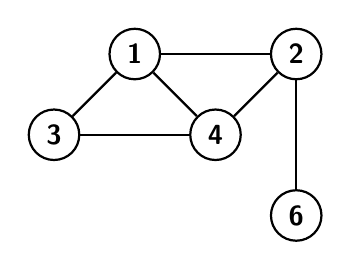
\begin{tikzpicture}[
    node distance=1.45cm, thick,
    main node/.style={circle, draw, font=\sffamily\bfseries}
]
    \node[main node] (1)                    {1};
    \node[main node] (3) [below left  of=1] {3};
    \node[main node] (4) [below right of=1] {4};
    \node[main node] (2) [above right of=4] {2};
    \node[main node] (6) [below right of=4] {6}; % <-4> forces an additional overlay in which node 2 disappears

    \path (1) edge (2)
        (4) edge (2)
        (6) edge (2);
    \path (1) edge (3)
        (4) edge (1);
    \path (3) edge (4);
\end{tikzpicture}
 \end{column}
 \pause
    \begin{column}{0.68\textwidth}
\begin{itemize}[<+->]
    \item Noder: $V={1,2,3,4,6}$
    \item Kanter: $E={(1,2), (1,4), (3,4), (2,4), (2,6), (1,3)}$
    \item Path: Vei fra A til B\\
    Eksempel: $Path(1,6)=(1,2,6)$
    \item Cycle: En path med samme start og slutt\\
    Eksempel: $(1,3,4,1)$, $(1,2,4,3,1)$
    \item Naboer: Set of noder som har en kante til en node\\
    Eksempel: $N(4)={1,2,3}$, $N(6)=2$
    \item Degree: Antall naboer av en node\\
    Eksempel: $deg(4)=3$, $deg(6)=1$
\end{itemize}
 \end{column}
\end{columns}
\end{frame}

\begin{frame}{}
    \begin{columns}
    \begin{column}{0.48\textwidth}
    \begin{figure}
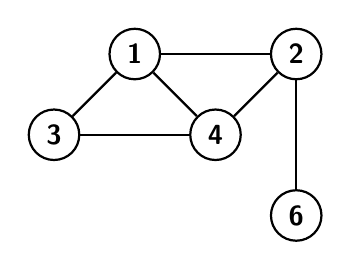
\begin{tikzpicture}[
    node distance=1.45cm, thick,
    main node/.style={circle, draw, font=\sffamily\bfseries}
]
    \node[main node] (1)                    {1};
    \node[main node] (3) [below left  of=1] {3};
    \node[main node] (4) [below right of=1] {4};
    \node[main node] (2) [above right of=4] {2};
    \node[main node] (6) [below right of=4] {6}; % <-4> forces an additional overlay in which node 2 disappears

    \path (1) edge (2)
        (4) edge (2)
        (6) edge (2);
    \path (1) edge (3)
        (4) edge (1);
    \path (3) edge (4);
\end{tikzpicture}
\caption{Urettet graf (undirected)}
\end{figure}
\begin{itemize}
    \item $deg(4) = 3$
\end{itemize}
 \end{column}
 \pause
    \begin{column}{0.48\textwidth}
    \begin{figure}
    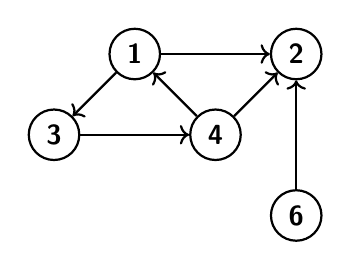
\begin{tikzpicture}[
    node distance=1.45cm, thick,
    main node/.style={circle, draw, font=\sffamily\bfseries}
]
    \node[main node] (1)                    {1};
    \node[main node] (3) [below left  of=1] {3};
    \node[main node] (4) [below right of=1] {4};
    \node[main node] (2) [above right of=4] {2};
    \node[main node] (6) [below right of=4] {6}; % <-4> forces an additional overlay in which node 2 disappears

    \path[->] (1) edge (2)
        (4) edge (2)
        (6) edge (2);
    \path[->] (1) edge (3)
        (4) edge (1);
    \path[->] (3) edge (4);
\end{tikzpicture}
\caption{Rettet graf (directed)}
\end{figure}
\begin{itemize}
    \item $deg^-(4) = 1$ (ingoing)
    \item $deg^+(4) = 2$ (outgoing)
\end{itemize}
 \end{column}
\end{columns}
\end{frame}

\begin{frame}
    \begin{block}{Bipartite graf $G(V,A,B)$}
    Set av nodene er delt i to sets $A,B$ der alle kanter $v\in V$ går fra en node i $A$ til en node i $B$\\
    Grafen kan farges i to farger med ingen to nabonoder i samme farge
    \end{block}

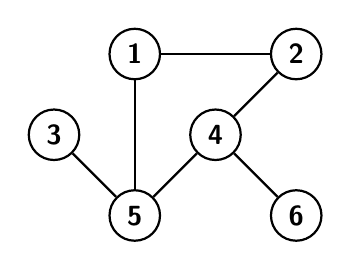
\begin{tikzpicture}[
    node distance=1.45cm, thick,
    main node/.style={circle, draw, font=\sffamily\bfseries}
]
    \node[main node,onslide=<2->{fill=black!40!green}] (1)                    {1};
    \node[main node,onslide=<2->{fill=black!40!green}] (3) [below left  of=1] {3};
    \node[main node,onslide=<2->{fill=black!40!green}] (4) [below right of=1] {4};
    \node[main node,onslide=<2->{fill=black!30!red}] (2) [above right of=4] {2};
    \node[main node,onslide=<2->{fill=black!30!red}] (5) [below right of=3] {5};
    \node[main node,onslide=<2->{fill=black!30!red}] (6) [below right of=4] {6};

    \path (1) edge (2)
        (1) edge (5)
        (3) edge (5)
        (4) edge (2)
        (4) edge (5)
        (4) edge (6);
\end{tikzpicture}
\end{frame}

\subsection*{Representasjon}
\begin{frame}
\begin{center}
\incomplete{5}{1/2,1/3,1/4,1/5,2/4,2/5}
\end{center}
\vspace{-1cm}
\begin{columns}
    \begin{column}{0.48\textwidth}
 \begin{table}[]
\centering
\label{tab:adjmatexample}
\begin{tabular}{r|ccccc}
  & 1 & 2 & 3 & 4 & 5 \\ \hline
1 & 0  & 1  & 1  &  1 & 1  \\
2 & 1  & 0  & 0  &  1 & 1  \\
3 & 1  & 0  & 0  &  0 & 0  \\
4 & 1  & 1  & 0  & 0  & 0  \\
5 & 1  & 1  & 0  & 0  & 0 
\end{tabular}
\caption{Adjacency matrix (directed)}
\end{table}
 \end{column}
    \begin{column}{0.48\textwidth}
\begin{table}[]
\centering
\label{tab:adjlistexample}
\begin{tabular}{r|l}
Node & Neighbours \\ \hline
1   &  {2,3,4,5}          \\
2   &  {1,4,5}          \\
3   &  {1}          \\
4   &  {1,2}          \\
5   &  {1,2}         
\end{tabular}
\caption{Adjacency list (directed)}
\end{table}
 \end{column}
\end{columns}
\end{frame}

\subsection{Trær}
\begin{frame}
\begin{block}{Tre $G(V,E)$}
    Et tre er en \textit{connected}, \textit{undirected} graph der ingen cycles eksisterer.
    \end{block}
    \pause
\begin{block}{Forest $G(V,E)$}
    En mengde av trær som ikke er tilknyttet med hverandre.
    \end{block}
    \pause
\begin{block}{Rooted tre $G(V,E)$}
    Et tre med en root node.
    \end{block}
\end{frame}

\begin{frame}
\begin{columns}
    \begin{column}{0.48\textwidth}
\begin{figure}
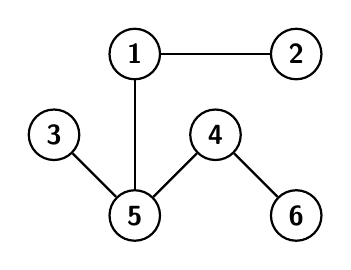
\begin{tikzpicture}[
    node distance=1.45cm, thick,
    main node/.style={circle, draw, font=\sffamily\bfseries}
]
    \node[main node] (1)                    {1};
    \node[main node] (3) [below left  of=1] {3};
    \node[main node] (4) [below right of=1] {4};
    \node[main node] (2) [above right of=4] {2};
    \node[main node] (5) [below right of=3] {5};
    \node[main node] (6) [below right of=4] {6};

    \path (1) edge (2)
        (1) edge (5)
        (3) edge (5)
        (4) edge (5)
        (4) edge (6);
\end{tikzpicture}
\caption{Et tre}
\end{figure}
 \end{column}
 \pause
    \begin{column}{0.48\textwidth}
\begin{figure}
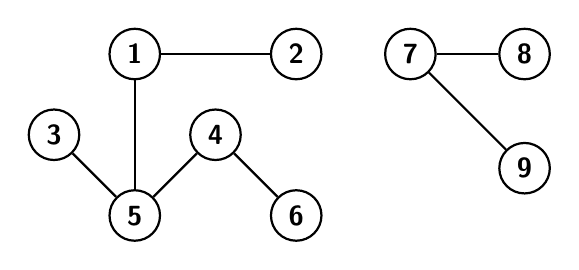
\begin{tikzpicture}[
    node distance=1.45cm, thick,
    main node/.style={circle, draw, font=\sffamily\bfseries}
]
    \node[main node] (1)                    {1};
    \node[main node] (3) [below left  of=1] {3};
    \node[main node] (4) [below right of=1] {4};
    \node[main node] (2) [above right of=4] {2};
    \node[main node] (5) [below right of=3] {5};
    \node[main node] (6) [below right of=4] {6};
    \node[main node] (7) [right of=2] {7};
    \node[main node] (8) [right of=7] {8};
    \node[main node] (9) [below of=8] {9};

    \path (1) edge (2)
        (1) edge (5)
        (3) edge (5)
        (4) edge (5)
        (4) edge (6)
        (7) edge (8)
        (7) edge (9);
\end{tikzpicture}
\caption{En skog (forest)}
\end{figure}
\end{column}
\end{columns}
\end{frame}

\begin{frame}{Rooted trees}
    \begin{block}{binary (m-ary) tre $G(V,E)$}
    Et tre med en root node der alle interne noder har eksakt to (m) barn.
    \end{block}
    \begin{columns}
    \begin{column}{0.48\textwidth}
\begin{figure}
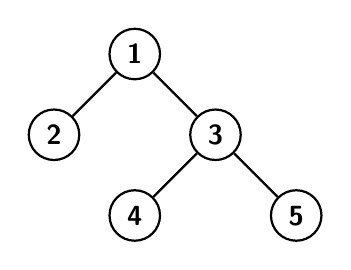
\begin{tikzpicture}[
    node distance=1.45cm, thick,
    main node/.style={circle, draw, font=\sffamily\bfseries}
]
   \node[main node] (1)                    {1};
    \node[main node] (2) [below left  of=1] {2};
    \node[main node] (3) [below right of=1] {3};
    \node[main node] (4) [below left of=3] {4};
    \node[main node] (5) [below right of=3] {5};

    \path (1) edge (2)
        (1) edge (3)
        (3) edge (4)
        (3) edge (5);
\end{tikzpicture}
\caption{binary tre}
\end{figure}
 \end{column}
    \begin{column}{0.48\textwidth}
\begin{figure}
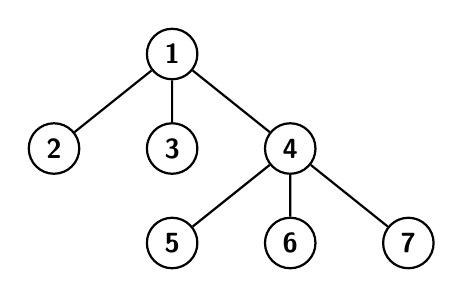
\begin{tikzpicture}[
    node distance=1.45cm, thick,
    main node/.style={circle, draw, font=\sffamily\bfseries},level distance=1.2cm,
  level 1/.style={sibling distance=1.5cm},
  level 2/.style={sibling distance=1.5cm}
]
  \node[main node] {1}
  	child {node[main node] {2}}
    child {node[main node] {3}}
    child {node[main node] {4}
    child {node[main node] {5}}
      child {node[main node] {6}}
    child {node[main node] {7}}
    };
\end{tikzpicture}
\caption{3-ary tre}
\end{figure}
\end{column}
\end{columns}
\end{frame}

\begin{frame}{Egenskaper}
    \begin{itemize}
        \item Et tre med $n$ noder har $n-1$ kanter
    \end{itemize}
   \begin{table}
    \begin{tabular}{l|l|l}
Noder & Interne noder & Leaves \\ \hline
\textbf{$n$} & $i=(n-1)/m$ & $l=((m-1)\cdot n+1)/m$\\
$n=m\cdot i + 1$ & \textbf{$i$} & $l=(m-1)\cdot i+1$\\
$n=(m\cdot l - 1)/(m-1)$ & $i=(l-1)/(m-1)$ & \textbf{$l$}          
\end{tabular}
\caption{Regne ut antall noder for fulle m-ary trær}
\end{table}
\end{frame}

\begin{frame}{Eksempel}
Et kjedebrev starter med en person som sender et brev til fem andre mennesker. Hver person som får et brev sender den enten videre til fem andre eller stopper å sende ting videre.\\
Gå ut ifra at 10.000 personer sender brevet videre og ingen får brevet to ganger.\\
(1) Hvor mange personer fikk et brev?\\
(2) Hvor mange sendte ikke brevet videre?\\\pause
\begin{itemize}
\item Folk som sender videre: Interne noder $i=10000$
\item Folk som ikke sender videre: Leaves $l = (5-1)\cdot 10000 + 1 = 40001$
\item Folk som fikk et brev: Noder $n=5\cdot 10000 + 1 = 50001$
\end{itemize}
\end{frame}

\subsection*{Spørretid}
\begin{frame}{Spørsmål?}
    \begin{figure}
        \centering
        \includegraphics[height = 4.9cm]{images/guillaume9.jpg}
        \caption{Guillaume foran Tvindefossen}
        \label{fig:guillaume9}
    \end{figure}
\end{frame}

\subsection{Algoritmer}
%\begin{frame}{Preorder Traversal}
%TODO: Fill with content @Lukas 
%\end{frame}
%
%\begin{frame}{Postorder Traversal}
%TODO: Fill with content @Lukas 
%\end{frame}
%
%\begin{frame}{Inorder Traversal}
%TODO: Fill with content @Lukas 
%\end{frame}

\begin{frame}{Spanning Trees}
	\begin{block}{Spanning Trees}
    Et Spanning Tree for en graf er et tree som besøker alle noder, men ikke lager cycles.
    \end{block}
    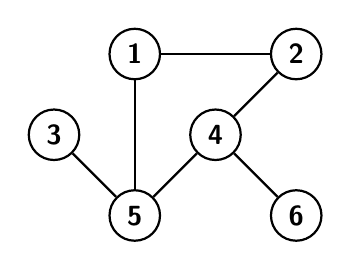
\begin{tikzpicture}[
    node distance=1.45cm, thick,
    main node/.style={circle, draw, font=\sffamily\bfseries}
]
    \node[main node] (1)                    {1};
    \node[main node] (3) [below left  of=1] {3};
    \node[main node] (4) [below right of=1] {4};
    \node[main node] (2) [above right of=4] {2};
    \node[main node] (5) [below right of=3] {5};
    \node[main node] (6) [below right of=4] {6};

    \path (1) edge (2)
        (1) edge (5)
        (3) edge (5)
        (4) edge (2)
        (4) edge (5)
        (4) edge (6);
\end{tikzpicture}
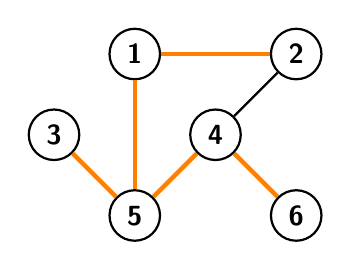
\begin{tikzpicture}[
    node distance=1.45cm, thick,
    main node/.style={circle, draw, font=\sffamily\bfseries}
]
    \node[main node] (1)                    {1};
    \node[main node] (3) [below left  of=1] {3};
    \node[main node] (4) [below right of=1] {4};
    \node[main node] (2) [above right of=4] {2};
    \node[main node] (5) [below right of=3] {5};
    \node[main node] (6) [below right of=4] {6};

    \path (1) edge[properties] (2)
        (1) edge[properties] (5)
        (3) edge[properties] (5)
        (4) edge (2)
        (4) edge[properties] (5)
        (4) edge[properties] (6);
\end{tikzpicture}
\end{frame}

\begin{frame}{Algoritmer for Spanning Trees}
Finne \textit{en} Spanning Tree
\begin{itemize}
\item Breadth-first search (BFS)
\item Depth-first search (DFS)
\end{itemize}
\hspace{1cm}

\noindent Finne \textit{en} Minimum Spanning Tree
\begin{itemize}
\item Prims algoritme
\item Kruskals algoritme
\end{itemize}
\end{frame}

\begin{frame}{BFS og DFS}
\begin{itemize}
\item Begge to går gjennom grafen fra en startnode
\item I hver runde går man videre til naboene til en node
\item Forskjell: BFS bruker kø, DFS stack
\item BFS: Rekkefølgen noder blir markert er rekkefølgen man går gjennom grafen
\item $\rightarrow$ Bredden blir utforsket før
\item DFS: Første noder som blir markiert er siste man ser på
\item $\rightarrow$ Algoritmen søker dypt først
\end{itemize}
\end{frame}

\begin{frame}[fragile]{Breadth-first search (BFS)}
\begin{minted}{python}
def bfs(graph):
   visited = [node] # alle besøkte noder
   queue = [node]   # køen
	
   while queue:     # så lenge noder er igjen
      m = queue.pop(0) # neste node 
      print(f"Visited: {m}")
      for neighbour in graph.neighbours(m): # gå gjennom naboer
         if neighbour not in visited:       # hvis ikke sett før
            visited += neighbour            # add til visited og kø
            queue += neighbour
\end{minted}
\end{frame}

\begin{frame}{Eksempel BFS}
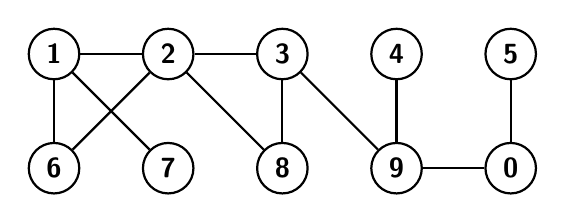
\begin{tikzpicture}[
    node distance=1.45cm, thick,
    main node/.style={circle, draw, font=\sffamily\bfseries}
]
    \node[main node] (1) [onslide=<1->{fill=black!30!red}]                   {1};
    \node[main node] (2) [right of =1,onslide=<2->{fill=black!30!red}] {2};
    \node[main node] (3) [right of =2,onslide=<3->{fill=black!30!red}] {3};
    \node[main node] (4) [right of =3,onslide=<5->{fill=black!30!red}] {4};
    \node[main node] (5) [right of =4,onslide=<6->{fill=black!30!red}] {5};
    \node[main node] (6) [below of =1,onslide=<2->{fill=black!30!red}] {6};
    \node[main node] (7) [right of =6,onslide=<2->{fill=black!30!red}] {7};
    \node[main node] (8) [right of =7,onslide=<3->{fill=black!30!red}] {8};
    \node[main node] (9) [right of =8,onslide=<4->{fill=black!30!red}] {9};
    \node[main node] (0) [right of =9,onslide=<5->{fill=black!30!red}] {0};

    \path (1) edge[onslide=<1->{propertiesBlue},onslide=<2->{propertiesRed}] (2)
        (1) edge[onslide=<1->{propertiesBlue},onslide=<2->{propertiesRed}] (6)
        (1) edge[onslide=<1->{propertiesBlue},onslide=<2->{propertiesRed}] (7)
        (2) edge[onslide=<2->{propertiesBlue},onslide=<3->{propertiesRed}] (3)
        (2) edge[onslide=<2->{propertiesBlue},onslide=<3->{propertiesRed}] (8)
        (3) edge (8)
		(3) edge[onslide=<3->{propertiesBlue},onslide=<4->{propertiesRed}] (9)
        (4) edge[onslide=<4->{propertiesBlue},onslide=<5->{propertiesRed}] (9)
        (9) edge[onslide=<4->{propertiesBlue},onslide=<5->{propertiesRed}] (0)
        (0) edge[onslide=<5->{propertiesBlue},onslide=<6->{propertiesRed}] (5)
        (2) edge (6);
\end{tikzpicture}
\medskip

\only<1>{
	Queue: 2 6 7
}
\only<2>{
	Queue: \cancel{2} \cancel{6} \cancel{7} 3 8
}
\only<3>{
	Queue: \cancel{2} \cancel{6} \cancel{7} \cancel{3} \cancel{8} 9
}
\only<4>{
	Queue: \cancel{2} \cancel{6} \cancel{7} \cancel{3} \cancel{8} \cancel{9} 4 0
}
\only<5>{
	Queue: \cancel{2} \cancel{6} \cancel{7} \cancel{3} \cancel{8} \cancel{9} \cancel{4} \cancel{0} 5
}
\only<6>{
	Queue: \cancel{2} \cancel{6} \cancel{7} \cancel{3} \cancel{8} \cancel{9} \cancel{4} \cancel{0} \cancel{5}
}
\end{frame}

\begin{frame}[fragile]{Depth-first search (DFS)}
\begin{minted}{python}
visited = []	# alle besøkte noder

def dfs(visited, graph, node):
   if node not in visited:      # hvis noden ikke er besøkt
      print(f"Visited: {node}") # markere som besøkt
      visited += node
      
      for neighbour in graph.neighbours(node): # gå gjennom naboer
         dfs(visited, graph, neighbour)        # rekursiv call
\end{minted}
\end{frame}

\begin{frame}{Eksempel DFS}
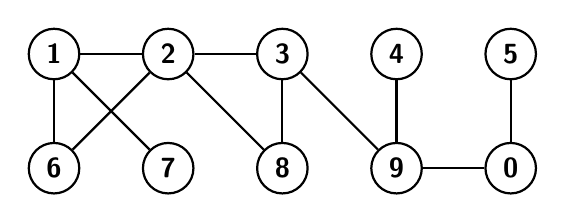
\begin{tikzpicture}[
    node distance=1.45cm, thick,
    main node/.style={circle, draw, font=\sffamily\bfseries}
]
    \node[main node] (1) [onslide=<1->{fill=black!30!red}]                   {1};
    \node[main node] (2) [right of =1,onslide=<3->{fill=black!30!red}] {2};
    \node[main node] (3) [right of =2,onslide=<4->{fill=black!30!red}] {3};
    \node[main node] (4) [right of =3,onslide=<7->{fill=black!30!red}] {4};
    \node[main node] (5) [right of =4,onslide=<9->{fill=black!30!red}] {5};
    \node[main node] (6) [below of =1,onslide=<11->{fill=black!30!red}] {6};
    \node[main node] (7) [right of =6,onslide=<12->{fill=black!30!red}] {7};
    \node[main node] (8) [right of =7,onslide=<5->{fill=black!30!red}] {8};
    \node[main node] (9) [right of =8,onslide=<6->{fill=black!30!red}] {9};
    \node[main node] (0) [right of =9,onslide=<8->{fill=black!30!red}] {0};

    \path (1) edge[onslide=<2->{propertiesBlue},onslide=<3->{propertiesRed}] (2)
        (1) edge[onslide=<2-11>{propertiesBlue}] (6)
        (1) edge[onslide=<2-11>{propertiesBlue},onslide=<12->{propertiesRed}] (7)
        (2) edge[onslide=<3-3>{propertiesBlue},onslide=<4->{propertiesRed}] (3)
        (2) edge[onslide=<3-9>{propertiesBlue}] (8)
        (3) edge[onslide=<4-5>{propertiesBlue},onslide=<5->{propertiesRed}] (8)
		(3) edge[onslide=<4-5>{propertiesBlue},onslide=<6->{propertiesRed}] (9)
        (4) edge[onslide=<6-6>{propertiesBlue},onslide=<7->{propertiesRed}] (9)
        (9) edge[onslide=<6-7>{propertiesBlue},onslide=<8->{propertiesRed}] (0)
        (0) edge[,onslide=<8-8>{propertiesBlue},onslide=<9->{propertiesRed}] (5)
        (2) edge[onslide=<3-10>{propertiesBlue},onslide=<11->{propertiesRed}] (6);
\end{tikzpicture}
\medskip

\only<1>{
	Stack: 
}
\only<2>{
	Stack: 7 6 2
}
\only<3>{
	Stack: 7 6 \cancel{2} 6 8 3
}
\only<4>{
	Stack: 7 6 \cancel{2} 6 8 \cancel{3} 9 8
}
\only<5>{
	Stack: 7 6 \cancel{2} 6 8 \cancel{3} 9 \cancel{8}
}
\only<6>{
	Stack: 7 6 \cancel{2} 6 8 \cancel{3} \cancel{9} \cancel{8} 0 4
}
\only<7>{
	Stack: 7 6 \cancel{2} 6 8 \cancel{3} \cancel{9} \cancel{8} 0 \cancel{4}
}
\only<8>{
	Stack: 7 6 \cancel{2} 6 8 \cancel{3} \cancel{9} \cancel{8} \cancel{0} \cancel{4} 5
}
\only<9>{
	Stack: 7 6 \cancel{2} 6 8 \cancel{3} \cancel{9} \cancel{8} \cancel{0} \cancel{4} \cancel{5}
}
\only<10>{
	Stack: 7 6 \cancel{2} 6 \cancel{8} \cancel{3} \cancel{9} \cancel{8} \cancel{0} \cancel{4} \cancel{5}
}
\only<11>{
	Stack: 7 6 \cancel{2} \cancel{6} \cancel{8} \cancel{3} \cancel{9} \cancel{8} \cancel{0} \cancel{4} \cancel{5}
}
\only<12>{
	Stack: \cancel{7} \cancel{6} \cancel{2} \cancel{6} \cancel{8} \cancel{3} \cancel{9} \cancel{8} \cancel{0} \cancel{4} \cancel{5}
}
\end{frame}

\begin{frame}{Minimum Spanning Trees}
\begin{block}{Minimum Spanning Trees}
    Et Minimum Spanning Tree for en graf er en Spanning Tree der summen av vektene (weights) er minimal.
    \end{block}
\begin{block}{Kruskals algoritme}
1. Sorter alle kanter etter sine vekter\\
2. Velg kanten med minst vekt som ikke ble valgt før. Hvis det nå blir en syklus, ignorer kanten. Hvis ikke, legg kanten til treet.\\
3. Repeter (2) så lenge til det er (n-1) kanter / alle noder er knyttet sammen.\\
\end{block}
\end{frame}


\begin{frame}{Eksempel Kruskal}
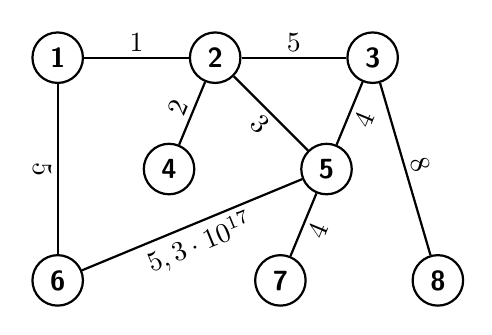
\begin{tikzpicture}[
    node distance=2cm, thick,
    main node/.style={circle, draw, font=\sffamily\bfseries},el/.style = {inner sep=2pt, align=left, sloped},
every label/.append style = {font=\tiny}
]
    \node[main node] (1) [onslide=<3->{fill=black!30!red}] {1};
    \node[main node] (2) [onslide=<3->{fill=black!30!red},right of =1] {2};
    \node[main node] (3) [onslide=<9->{fill=black!30!red},right of =2] {3};
    \node[main node] (4) [onslide=<5->{fill=black!30!red},below right of =1] {4};
    \node[main node] (5) [onslide=<7->{fill=black!30!red},below right of =2] {5};
    \node[main node] (6) [onslide=<15->{fill=black!30!red},below left of =4] {6};
    \node[main node] (7) [onslide=<11->{fill=black!30!red},below right of =4] {7};
    \node[main node] (8) [onslide=<17->{fill=black!30!red},below right of =5] {8};
    
    \path (1)  edge[onslide=<2-2>{propertiesBlue},onslide=<3->{propertiesRed}] node[el,above]  {1}  (2)
     (2)  edge[onslide=<12-12>{propertiesBlue},onslide=<13->{propertiesGrey}] node[el,above]  {5}  (3)
     (1)  edge[onslide=<14-14>{propertiesBlue},onslide=<15->{propertiesRed}] node[el,below]  {5}  (6)
     (2)  edge[onslide=<4-4>{propertiesBlue},onslide=<5->{propertiesRed}] node[el,above]  {2}  (4)
     (2)  edge[onslide=<6-6>{propertiesBlue},onslide=<7->{propertiesRed}] node[el,below]  {3}  (5)
     (3)  edge[onslide=<8-8>{propertiesBlue},onslide=<9->{propertiesRed}] node[el,below]  {4}  (5)
     (5)  edge[onslide=<10-10>{propertiesBlue},onslide=<11->{propertiesRed}] node[el,below]  {4}  (7)
     (3)  edge[onslide=<16-16>{propertiesBlue},onslide=<17->{propertiesRed}] node[el,above]  {8}  (8)
     (6)  edge[onslide=<18->{propertiesGrey}] node[el,below]  {$5,3\cdot 10^{17}$}  (5);
\end{tikzpicture}

\end{frame}

%\section*{Slutt}
\begin{frame}
\begin{center}
\begin{Large}
\textbf{Lykke til på eksamen!\\[5mm]
Takk for oss :)}

\end{Large}
\end{center}  
\end{frame}
\end{document}